\documentclass[german]{latex4ei/latex4ei_sheet}

\usepackage{xcolor}
\usepackage{enumitem}
\usepackage{stackengine,xcolor,scalerel}

\def\cpm{\mathbin{\ensurestackMath{\abovebaseline[-2.5pt]{%
  \stackunder[-2.4pt]{\color{red}+}{\color{green}-}}}}}

\newcommand\equalhat{\mathrel{\stackon[1.5pt]{=}{\stretchto{%
                \scalerel*[\widthof{=}]{\wedge}{\rule{1ex}{3ex}}}{0.5ex}}}}

\titlespacing*{\subsection}{.5pt}{.5pt}{2pt}
\titlespacing*{\subsubsection}{0pt}{.5pt}{2pt}

\begin{document}

\section{Klassische Mechanik}
\begin{sectionbox}
    \subsection{Bewegungen}

    \subsubsection{Freier Fall}
    $h=\frac{1}{2}gt^2 \qquad v_E=\sqrt{2gh_0}$\\
    $\Delta t = \sqrt{2h/g}$

    \subsubsection{Senkrechter Wurf}
    $h=v_0t-\frac{1}{2}gt^2+h_0$\\
    $v_M=\sqrt{\frac{1}{2}v_0} \qquad v^2 = v_0^2-2g(h_0-h)$\\
    $v=v_0-g  t$\\
    $t_{h,\ir max}=\frac{v_0}{g} \qquad h_{\ir max}=\frac{v_0^2}{2g}$

    \subsubsection{Waagrechter Wurf}
    $t_{\ir Fall}=\sqrt{\frac{2h_0}{g}}$ \\
    $y(t)=h_0-\frac{1}{2}gt^2 \qquad x(t)=v_0  t$\\
    $v_y=gt \qquad v_x = v_0$\\
    $y(x)=h_0-\frac{g  x^2}{2v_0^2}$

    \subsubsection{Schräger Wurf}
    $v_x=v_0\cos \alpha \qquad v_y=v_0\sin \alpha -gt$\\
    $v(\Delta h)=\sqrt{v_0^2-2g\Delta h}$\\
    $x=v_0t\cos \alpha \qquad y=v_0t \sin \alpha - \frac{1}{2} gt^2 +h_0$\\
    $x_{\ir max}=\frac{v_0^2 \sin{(2\alpha)}}{g}$\\
    $t_{\ir Wurf}=\frac{2v_0\sin \alpha}{g}$ \quad
    $t_{h,\ir max}=\frac{1}{2}t_{\ir Flug}$ \quad
    $h_{\ir max}=\frac{v_0^2 \sin^2 \alpha}{2g}+h_0$ \\

    % \subsubsection{Schiefe Ebene}
    % $F_H=F_G \sin \alpha \qquad F_N=F_G\sin\alpha$ \\
    % $F_{HR}=\mu_{HR}F_N \qquad F_{GL} = \mu_{GL}F_N$ \\

    \begin{cookbox}{Newton'sche Axiome}
        \item Masse ist träge. Jeder Körper behält seinen Bewegungszustand bei.
        \item $\vec F=m\vec a=\dot{\vec p}$
        \item $\vec F_{12}=-\vec F_{21}$
    \end{cookbox}
\end{sectionbox}


\begin{sectionbox}
    \subsection{Kraft, Energie, Impuls}
    \subsubsection{Kraft}
    \begin{tablebox}{ll}
        Federkraft & $\vec F_F=-kx$ \\ & $x:$ Auslenkung vom GGP \\
        Gewichtskraft & $F_G=mg$ \\
        & $F_N=mg\cos \alpha$ \\
        & $F_H=mg\sin \alpha$ \\
        Zentripetalkraft & $F_Z=ma_{Z}=m \frac{v^2}{r}=m\omega^2r=p\omega$ \\
        & Zeigt in Richtung Mittelpunkt des Kreises von \\ & einem sich nicht rotierenden Beobachter \\
        Zentrifugalkraft & $F_{\it flieh}=-F_Z$ \\
        & Zeigt vom Mittelpunkt des Kreises weg. Der Beobachter \\ & rotiert sich hier mit ($\rightarrow$ Scheinkraft) \\
        Reibungskraft & $F_R=\mu F_{(N)}=\mu m g   \cos \alpha$
    \end{tablebox}
    \subsubsection{Energie}
    \begin{tabular}{c|c}
        $E_{\ir kin}=\frac{1}{2}mv^2=\frac{p^2}{2m}$ & $E_{\ir pot}=mgh$                  \\
        $E_{F}=\frac{1}{2}kx^2$                      & $E_{\ir rot}=\frac{1}{2}I\omega^2$
    \end{tabular}

    \subsubsection{Arbeit}
    $W=\Delta E=\vec F \vec s=|\vec F| \, |\vec s|\cos\alpha$
    \subsubsection{Leistung}
    $P=
        \underbrace{\frac{\Delta W}{\Delta t}}_{\text{mittlere Leistung}}
        = \, \underbrace{\frac{F  \Delta s}{\Delta t}=F  v}_{\text{momentane Leistung}}$\\
    $\eta=\frac{E_{\it nutz}}{E_{\ir zu}}=\frac{P}{P}$
    \subsubsection{Impuls}
    $p_{\ir vorher}=p_{\ir nachher} \qquad p=mv$
    \begin{tablebox}{ll}
        Mittlere Kraft     & $\overline{F}=\frac{\Delta p}{\Delta t}$\\
        Elastischer Stoß   & $m_1v_1+m_2v_2=m_1u_1+m_2u_2$\\
        & $E_{\ir kin,ges}=$ const. \\
        Unelastischer Stoß & $m_1v_1+m_2v_2=(m_1+m_2)u$ \\
        & $E_{\ir kin,ges}\ne$ const.
    \end{tablebox}
    \subsubsection{Raketengleichung}
    TODO
\end{sectionbox}


\begin{sectionbox}
    \subsection{Rotation}
    \begin{tabular}{l|ll}
        Kinematik       & Rotation                & Einheit[Rot.]            \\ \hline
        Masse $m$       & Trägheitsmoment $I$/$J$ & $[I]=kgm^2$              \\
        Impuls $\vec p$ & Drehimpuls $\vec L$     & $[L]=\frac{kgm^2}{s}=Js$ \\
        Kraft $\vec F$  & Drehmoment $\vec M$     & $[M] = Nm$
    \end{tabular}

    \subsubsection{Bewegungsgleichungen}
    \begin{tabular}{ll}
        Winkel                & $\varphi(t)=\omega t$ bei $\omega=\text{const.}, \alpha = 0$                 \\
                              & $\varphi(t)=\frac{1}{2} \alpha t^2$ bei $\alpha=\text{const.}$               \\
        Winkelgeschwindigkeit & $\omega = \frac{2\pi}{T}=\frac{\Delta \varphi}{\Delta t}$                    \\
                              & $\vec \omega = \frac{\vec r \times \vec v}{r^2}$ (in Richtung der Rot.achse) \\
        Winkelbeschleunigung  & $\alpha = \frac{\Delta \omega}{\Delta t}$                                    \\
        Bahngeschwindigkeit   & $\vec v = \vec \omega \times \vec r$
    \end{tabular}

    \subsubsection{Trägheitsmoment $I$ oder $J$}
    \begin{tablebox}{lll}
        Zylindermantel & $I = mr^2$ & Drehachse ist Körperachse\\
        Hohlzylinder & $I = \frac{1}{2}m(r_a^2+r_i^2)$ & Drehachse ist Körperachse\\
        Massive Kugel & $I = \frac{2}{5}mr^2$  & Drehachse durch Mittelpunkt\\
    \end{tablebox}
    TODO: Satz von Steiner

    \subsubsection{Drehimpuls}
    $\vec L=\vec r\times \vec p = \vec r \times m\vec v = I \vec \omega$ \\
    Immer im Bezug auf Ursprung von $\vec r$ mit $\vec r$: Abstand von der Drehachse

    \subsubsection{Drehmoment (analog zu Kraft)}
    $\vec M=\vec r\times \vec F=|\vec F| \, |\vec r|  \sin \alpha$\\
    $\vec M=I  \dot{\vec{\omega}}=I\vec \alpha=\frac{\partial \vec L}{\partial t}$
\end{sectionbox}

\begin{sectionbox}
    \subsection{Corioliskraft}
    \begin{emphbox}
        $\vec{F_c}=2m(\vec v\times \vec \omega)= 2m v w   \sin{(v\angle \omega)}$
    \end{emphbox}
    $\vec v$: Bewegungsrichtung, $\vec w$: (Richtung der) Rotationsachse, senkrecht zur Rotationsrichtung (auf der Erde nach Norden)\\
    $a_c=-2(\omega \times v)=2v\omega$\\
    $\Delta x= \frac{2}{3}\cos (\beta) \omega h \sqrt{\frac{2h}{g}}$\\
    $\Delta y = -\omega^2R\cos (\beta) \sin (\beta) \frac{h}{g}$\\
    %
\includegraphics[width=0.25\columnwidth]{coriolis.pdf}
    $R_E=\SI{6370}{\kilo \meter} \qquad r=R_E \cos \varphi \qquad \omega_E=\frac{2\pi}{86400\si{\second}}$\\
    $F_C$: Auf der Nordhalbkugel nach rechts. Auf der Südhalbkugel nach links.
\end{sectionbox}

\begin{sectionbox}
    \subsection{Planetenbewegungen}
    \subsubsection{Gravitation}
    $E_{\ir pot}=-G\frac{m_E  m}{r} \qquad r>r_E$\\
    $\vec{F}_G=G\frac{m_1m_2}{r^2}  \vec{e_r}$\\
    $g=G  \frac{m}{r^2}$\\
    $W_G=Gm_1m_2(\frac{1}{r_1}-\frac{1}{r_2})$\\
    $F_G \, || \, r \rightarrow M=r\times F=0$\\

    Satellit-Erde: $\frac{1}{2}m_Sv^2=G\frac{m_Sm_E}{R_E}$ \\
    Stabile Umlaufbahn: $\omega_S=\sqrt{\frac{G  m_E}{r^3}}\qquad v=\omega r$\\
    Geostat. Umlaufbahn: $r_g=\sqrt[3]{G  m_E   \frac{T_g^2}{4\pi^2}} \qquad h_g=r_g-R_E$

    TODO: Keplersche Gesetze?
\end{sectionbox}

\section{Schwingungen}
\begin{sectionbox}
    \subsection{Frei ungedämpft}
    \textbf{Bewegungsgleichung}: $\ddot{x}+\omega_0^2x=0$\\
    $f_0=\frac{\omega_0}{2\pi} \qquad y_0=\frac{mg}{k} \qquad v_0 = \hat{x}\sqrt{\frac{k}{m}}$

    \subsubsection{Federpendel}
    $x(t)=x_{\ir max}\cos (\omega_0 t + \varphi_0) \qquad \omega_0 = \sqrt{\frac{k}{m}}$\\
    $x_{\ir max}=\sqrt{x_0^2+(\frac{v_0}{\omega_0})^2}$\\
    Bewegungsgleichung: $\ddot{x}+\frac{k}{m}x=0$

    \subsubsection{Fadenpendel}
    $x(t)=x_{\ir max}\cos (\omega_0 t + \varphi_0) \qquad \omega_0 = \sqrt\frac{g}{l}$\\
    $l=\frac{T^2g}{4\pi^2} \qquad h=l-l\cos \alpha$\\
    $x_{\ir max}=\sqrt{x_0^2+(\frac{v_0}{\omega_0})^2} \qquad E_{\ir ges} = mgl(\frac{3}{2}-\cos \alpha)$\\
    Bewegungsgleichung: $\ddot{\theta}+\frac{g}{l}\theta=0$

    \subsubsection{Torisionsschwingungen (Drehpendel) (TODO: s. Übung 9)}
    $\theta(t)=\theta_{\ir max}\cos(\omega_0 t + \varphi_0)$ \\
    $\omega_0 = \sqrt{\frac{k_t}{I}}=\sqrt{\frac{k_t}{mr^2}}$\\
    $I=\frac{T^2}{4\pi^2}k_t \qquad T_0=2\pi \sqrt{\frac{I}{k_t}}$\\
    Bewegungsgleichung: $\ddot{\theta}+\frac{k_t}{I}\theta=0$
\end{sectionbox}

\begin{sectionbox}
    \subsection{Frei gedämpft}
    \begin{tablebox}{ll}
        Stokesche Reibungskraft & $\vec F_R=-6 \pi \eta R \vec{v}=-2m\gamma\vec{v}$\\
        Resonanzfreq./gedämpfte Eigenfreq. & $\omega_D=\sqrt{\omega_0^2-\gamma^2}$ \\
        Bewegungsgleichung & $\ddot{x}+2\gamma \dot{x}+\omega_0^2x=0$
    \end{tablebox}
    $\gamma = \frac{\delta}{2m}=\frac{3\pi \eta R}{m} \quad \text{Reibungsterm/Abklingkoeffizient}, [\gamma] = \frac{1}{s}$ \\
    $\delta$: Dämpfungskonstante

    \subsubsection{Schwingfall (geringe Reibung) $\omega_0^2>\gamma^2$}
    $\omega_D=\sqrt{\omega_0^2-\gamma^2}<\omega_0$\\
    $x(t)=Ae^{-\gamma t}\cos(\omega_Dt)$

    \subsubsection{Aperiodischer Grenzfall $\omega_0^2=\gamma^2$}
    $\omega_D=0$\\
    $x(t)=Ae^{-\gamma t}  (1+\gamma t)$

    \subsubsection{Kriechfall (starke Reibung) $\omega_0^2<\gamma^2$}
    $\omega_D=i\gamma \pm i\sqrt{\gamma^2-\omega_0^2}$\\
    $x(t)=A_1e^{-\big(\gamma+\sqrt{\gamma^2-\omega_0^2}\big)t}+A_2e^{-\big(\gamma - \sqrt{\gamma^2-\omega_0^2}\big)t}$\\
\end{sectionbox}

\begin{sectionbox}
	\subsection{Erzwungen gedämpft}
    Gedämpfte Schwingung, die durch eine weitere Kraft dazu gezwungen wird, in Schwingung zu bleiben.
	Nach der Einschwungzeit soll das System mit der Kreisfrequenz $\Omega$ schwingen. \\

    \begin{tablebox}{ll}
        Resonanzfrequenz & $\Omega_{\ir res}=\sqrt{\omega_0^2-2\gamma^2}$ \\
        Bewegungsgleichung & $\ddot{x}+2\gamma \dot{x}+\omega_0^2x=\underbrace{F_0e^{-i\Omega t}}_{\text{externe Kraft}}$
    \end{tablebox}

    Auslenkung: $A = \frac{F_0}{m}\frac{1}{\sqrt{(\omega_0^2-\Omega^2)^2+4\gamma^2\Omega^2}}$ \\
    Phasenverschiebung: $\tan\varphi = \frac{2\gamma\Omega}{\omega_0^2-\Omega^2}$

    \begin{cookbox}{Resonanzfälle}
		\item $\Omega < \omega_0$ (Langsame Erregerfrequenz) \\
		$A\rightarrow \frac{F_0}{m\omega_0^2}=\frac{F_0}{k}$\qquad
		$\Delta \varphi = 0 \qquad \Omega \rightarrow 0$
		
        \item $\Omega \approx \omega_0$ (Katastrophe, Resonanz) für $\gamma \rightarrow 0$ \\
		$A_{\ir max}=\frac{F_0}{2m\gamma \omega_D} \rightarrow \frac{F_0}{\delta\omega_0} \rightarrow \infty$\\
		$\Omega_{\ir max}=\omega_D \rightarrow \omega_0 \qquad \Delta \varphi = \frac{\pi}{2}$
		
        \item $\Omega > \omega_0$ (Schnelle Erregerfrequenz) \\
		$\Delta \varphi = \pi \qquad \Omega \rightarrow \infty \qquad A\rightarrow 0$
	\end{cookbox}
    
\end{sectionbox}

\section{Wellen}
\begin{sectionbox}
    \subsection{Allgemeines}
    \textbf{Allgemeine Wellengleichung:} $\frac{1}{c^2}\frac{\partial^2u}{\partial t^2}=\Delta u$\\

    $c=\lambda   f=\frac{\omega}{k}=\frac{x}{\Delta t}$\\
    $k=\frac{2\pi}{\lambda}=\frac{\omega}{c} \qquad \text{Wellenzahl}$ \\

    \subsubsection{Laufende Welle}
    \begin{emphbox}
        \textbf{Funktion:} $y(x,t)=y_{\ir max}\sin(kx \cpm \omega t + \varphi_0)^{\textcolor{red}{\text{+: Welle in neg. x}}}_{\textcolor{green}{\text{-: Welle in pos. x}}}$
    \end{emphbox}

    \subsubsection{Stehende Welle}
    Oberschwingung: $n$, ($n=0$ für $0$-te Schwingung $\rightarrow$ ein Bauch) \\
    Stablänge: $L=\frac{(2n+1)\lambda}{2}$ \\
    Grundfrequenz: $f_0=\frac{c}{2L}$ \\
    Frequenzen der Oberschwingungen: $f_n=(2n+1)f_0$
\end{sectionbox}

\begin{sectionbox}
    \subsection{Doppler-Effekt}
    \begin{cookbox}{}
        \item Beobachter \textbf{bewegt}, Quelle \textbf{ruht}\\
        \begin{itemize}
            \item[] $f_B=f_Q(1\cpm\frac{v_B}{c})^{\textcolor{red}{\text{+: Annäherung}}}_{\textcolor{green}{\text{-: Entfernung}}}$\\
        \end{itemize}
        \item Beobachter \textbf{ruht}, Quelle \textbf{bewegt}\\
        \begin{itemize}
            \item[] $f_B=\frac{f_Q}{1\cpm v_Q/c}^{\textcolor{red}{\text{+: Entfernung}}}_{\textcolor{green}{\text{-: Annäherung}}}$\\
        \end{itemize}
        \item Beobachter \textbf{bewegt}, Quelle \textbf{bewegt}\\
        $f_B = f_Q \frac{c \, \underset{\textcolor{green}{-}}{\textcolor{red}{+}} \, V_B}{c \, \underset{\textcolor{green}{+}}{\textcolor{red}{-}} \, V_Q} \qquad \text{Q} \, \underset{\textcolor{green}{\leftarrow} \textcolor{green}{\rightarrow}}{\textcolor{red}{\rightarrow} \textcolor{red}{\leftarrow}} \, \text{B}$\\
        $f_B = f_Q \frac{c \, \underset{\textcolor{cyan}{-}}{\textcolor{purple}{+}} \, V_B}{c \, \underset{\textcolor{cyan}{-}}{\textcolor{purple}{+}} \, V_Q} \qquad \text{Q} \, \underset{\textcolor{cyan}{\rightarrow} \textcolor{cyan}{\rightarrow}}{\textcolor{purple}{\leftarrow} \textcolor{purple}{\leftarrow}} \, \text{B}$\\
        \item Quelle \textbf{bewegt} (TODO) ($v>1 \, \ir Ma$)\\
        $\sin \alpha=\frac{\diff w}{\diff s}=\frac{c_s t}{v_Qt}=\frac{1}{\ir Ma}$
    \end{cookbox}
\end{sectionbox}


\begin{sectionbox}
    \subsection{Interferenz}
    \subsubsection{Einfachspalt (Beugung)}
    $b$: Spaltbreite \\
    Gangunterschied: $\Delta s = b\sin\alpha \approx \frac{x}{D}b$ \\
    Maxima: $\Delta s=\pm (m + \frac{1}{2})\lambda$ \\
    Minima: $\Delta s=\pm m\lambda \rightarrow x_{\ir min} \approx \pm\frac{m\lambda D}{b} \qquad m = (1,2,...,n)$ \\

    \subsubsection{Doppelspalt}
    $d$: Spaltenabstand, $D$: Abstand zum Schirm, $m = (0,1,...,n)$ \\
    Gangunterschied: $\Delta s = d\sin\alpha \approx \frac{x}{D}d$ \\
    Phasenunterschied: $\Delta\varphi = 2\pi \frac{\Delta s}{\lambda}$ \\
    Konstr. Int. (Maxima): $\Delta s=\pm m\lambda \rightarrow x_{\ir max}\approx\pm\frac{m\lambda D}{d}$ \\
    Destr. Int. (Minima): $\Delta s = \pm (m - \frac{1}{2})\lambda \rightarrow x_{\ir min}\approx \pm (m - \frac{1}{2})\frac{\lambda D}{d}$ \\

    \subsubsection{Gitter}
    $d$: Spaltenabstand, $D$: Abstand zum Schirm, $m = (0,1,...,n)$ \\
    Gangunterschied: $\Delta s = d\sin\alpha \approx \frac{x}{D}d$ \\
    Hauptmaxima: $\Delta s=\pm m\lambda \rightarrow x_{\ir max}\approx\pm\frac{m\lambda D}{d}$ \\
    Nebenmaxima: $\Delta s = \pm \frac{2k + 1}{2N}\lambda$\\
    Abstand benachbarter Maxima $\Delta x \approx \frac{\lambda D}{d}$ \\

    \subsubsection{An dünner Schicht $n_2 > n_1$}
    $d$: Dicke der Schicht, $\alpha$: Einfallswinkel \\
    $\Delta s = 2d \sqrt{n_2^2-n_1^2\sin^2\alpha} + \frac{\lambda}{2}$ \\
    Maxima und Minima wie beim Doppelspalt
\end{sectionbox}

\section{Optik}
\begin{sectionbox}
    \subsection{Rexlexion und Brechnung}
    $f_{\text{Medium}}\lambda_{\text{Medium}} = c_{\text{Medium}} \qquad \lambda_{\text{Medium}} = \frac{\lambda_{\text{Vakuum}}}{n}$\\
    Berchnungsindex $n=\frac{c_\text{Vakuum}}{c_{\text{Medium}}}$
    \subsubsection{Brechung}
    \begin{emphbox}
        \textbf{Gesetz von Snellius:}
        $\frac{\sin \alpha}{\sin \beta} = \frac{n_2}{n_1} = \frac {c_1}{c_2}$
    \end{emphbox}
    \begin{enumerate}
        \item[A)] \textbf{zum Lot} (dünn nach dicht)\\
              $\sin \alpha > \sin \beta$ \qquad $c_1 > c_2$
        \item[B)] \textbf{vom Lot} (dicht nach dünn)\\
              $\sin \alpha < \sin \beta$ \qquad $c_1 < c_2$
    \end{enumerate}
    \subsubsection{Totalreflexion}
    Nur möglich wenn $n_1 > n_2$ und $\theta > \theta_{\ir krit}$ \\
    $\theta_{\ir krit} = \arcsin \frac{n_2}{n_1}$\\
    Einfallswinkel = Ausfallswinkel
\end{sectionbox}

\begin{sectionbox}
    \subsection{Linsen}
    \begin{tablebox}{ll}
        Linsengleichung &
        $D=\frac{1}{f}=\frac{1}{g}+\frac{1}{b}$\\
        Vergößerung & $V=\frac{B}{G}= - \frac{b}{g}=\frac{\tan \alpha}{\tan \alpha_0}$\\
    \end{tablebox}
    $g>0$ links der Linse, $b>0$ rechts der Linse \\
    Falls $b<0 \Rightarrow$ virtuelles Bild \\
    Falls $V < 0$: Bild nach unten geklappt \\
    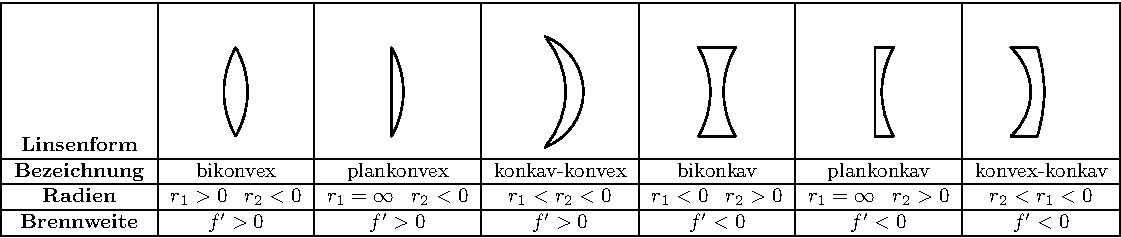
\includegraphics[width=\columnwidth]{img/Linsen_crop.pdf}

    \subsubsection{Hohlspiegel}
    $f=\frac{r}{2}$ \qquad $V=\frac{B}{G}= - \frac{n_1b}{n_2g}$ \\
    $D=\frac{n_1}{g}+\frac{n_2}{b}=\frac{n_2-n_1}{r}$\\
    $g\rightarrow \infty: b=f_B=\frac{n_2r}{n_2-n_1}$\\
    $b\rightarrow \infty: g=f_G=\frac{n_1r}{n_2-n_1}$\\

    \subsubsection{Dünne Linsen}
    $\frac{1}{f}=\frac{1}{g}+\frac{1}{b}=(\frac{n_2}{n_1}-1)(\frac{1}{r_1}-\frac{1}{r_2})$\\
    mit $r_1$ Krümmungsradius der linken Linse, $r_2$ Krümmungsradius der rechten Linse (bei rechtskonvex ist $r_2<0$)

    \paragraph{Konvexe Linse (Sammellinse)}
    Korrektur von Weitsichtigkeit \\
    $V_{\ir sammel}= \frac{b}{g}=\frac{b-f}{f}$\\

    Abbildung:
    \begin{tablebox}{lcllr}
        $\infty > g > 2f $ & $\Rightarrow$ & $2f>b>f$ & $G>B$ & real und invertiert\\
        $g=2f $ & $\Rightarrow$ & $2f=b$ & $G=B$ & real und invertiert\\
        $2f>g>f $ & $\Rightarrow$ & $ \infty >b>2f$ & $G<B$ & real und invertiert\\
        $0<g<f $ & $\Rightarrow$ & $ -b>g$ & $G<B$ & virtuell und aufrecht\\
    \end{tablebox}
    \paragraph{Konkave Linse (Zerstreuungslinse)}
    Korrektur von Kurzsichtigkeit\\
    Abbildung:
    \begin{itemize}
        \item[$\rightarrow$] Bild immer zwischen Brennpunkt und Linse
        \item[$\rightarrow$] Bild immer verkleinert ($G>B$)
        \item[$\rightarrow$] Bild immer virtuell und aufrecht
    \end{itemize}

    \subsubsection{Dicke Linsen}
    $\frac{1}{f}=(\frac{n}{n_0}-1)\cdot(\frac{1}{r_1}-\frac{1}{r_2}+\frac{(n-n_0)d}{n \cdot r_1 r_2})$\\
    $h_1=-\frac{f(n-1)d}{n \cdot r_2}$ \qquad $h_2=-\frac{f(n-1)d}{n \cdot r_1}$

    \subsubsection{Linsensysteme}
    \begin{itemize}
        \item \textbf{Lochkamera} \\
              $S=\frac{D(b+g)}{g}$
        \item \textbf{Lupe} \\
              $V=\frac{\tan \alpha_L}{\alpha_0}=\frac{G/f}{G/s_0}=\frac{s_0}{f}$ mit $s_0=\SI{25}{\centi \meter}$
        \item \textbf{Fernrohr} \\
              $V=\frac{f_{ob}}{f_{ok}}$, $g\approx \infty$, $b\approx f$ \\
              $V_T=\frac{f}{g-f}=\frac{b-f}{f}\approx 0$
        \item \textbf{Mikroskop} \\
              $V=V_{ok}\cdot V_{ob}=\frac{(d-f_{ob})s_0}{f_ob \cdot f_ok}=-\frac{l}{f_{ob}}\cdot \frac{s_0}{f_{ok}}$
        \item \textbf{Auflösung Mikroskop} \\
              mit Spalt b: $\delta_{\ir{min}} = \alpha = \arcsin\frac{\lambda}{b} \approx \frac{\lambda}{b}$ (Abbé Limit)\\
              für runde Linse mit Durchmesser D: $\delta_{\ir{min}} = D\cdot\sin\alpha = 1,22\frac{\lambda}{D}$ (Rayleigh-Kriterium)\\
    \end{itemize}
\end{sectionbox}

\begin{sectionbox}
    \subsection{Absorption}
    Berchungsindex mit Absorption: $n\rightarrow \tilde{n}=n-i\kappa$\\
    Re($\tilde{n}$)$=n$: Brechung \\
    Im($\tilde{n}$)$=\kappa$: Absorption \\

    \begin{emphbox}
        \textbf{Absorptionsgesetz} von Lambert-Beer: $I=I_0e^{-\alpha \cdot d}=I_0e^{-\frac{2\omega}{c}\kappa d}$
    \end{emphbox}

    \subsubsection{Polarisation}
    \begin{emphbox}
        \textbf{Gesetz von Malus} (für polarisiertes Licht): $I = I_0 \cos^2 \alpha$
    \end{emphbox}
    Für unpolarisiertes Licht gilt nach einem Polarisationsfilter: $I = \frac{I_0}{2}$
\end{sectionbox}


\section{Hydromechanik}
\begin{sectionbox}
	\subsection{Allgemein}
	\begin{tablebox}{ll}
		Volumen & $1l \equalhat 10^{-3}m^3$ \\
		Druck   & $1bar \equalhat 100000Pa$ \\
		Dichte  & $\rho=\frac{m}{V}$ \\
		Reynolds-Zahl & $R_E= \frac{\rho vd}{\eta}$ \\
		& $R_E < R_{E,krit.}$ laminar (z.B. Wasser) \\
		&	$R_E > R_{E,krit.}$ turbulent (z.B. Honig)
	\end{tablebox}
\end{sectionbox}

\begin{sectionbox}
	\subsection{Hydraulische Presse}
	für sich nicht bewegende Flüssigkeiten. Man drückt einen Kolben hinein und ein anderer bewegt sich heraus (z.b. Baggerarm)
	\begin{emphbox}
		$\frac{F_1}{A_1}=\frac{F_2}{A_2}$
	\end{emphbox}
	$\frac{\Delta x_1}{\Delta x_2}=\frac{F_2}{F_1}=\frac{A_2}{A_1}$ mit $\Delta x$: Verschiebung (Hubweg) der Kolben
\end{sectionbox}

\begin{sectionbox}
	\subsection{Kontinuitätsgleichung}
	für sich bewegende Flüssigkeiten (z.B. Wasser im Gartenschlauch wird durch kleine Düsen gedrückt)
	\begin{emphbox}
		$\dot{m}=\rho_1 A_1 \vec{v_1}=\rho_2 A_2 \vec{v_2}$
	\end{emphbox}
	$\dot{V}=\frac{\dot{m}}{\rho}=A\vec{v}$
\end{sectionbox}

\begin{sectionbox}
	\subsection{Bernoulli Gleichung}
	Beschreibt den Gesamtdruck eines Punktes. Dieser setzt sich zusammen aus dem statischen Druck (z.B. atmosphärischer Druck), dem Druck aufgrund einer sich bewegenden Flüssigkeit und dem Druck aufgrund einer Menge an Wasser (z.B. $10m$ unter Wasser)
	\begin{emphbox}
		$p_{\ir ges}=\underbrace{p}_{\text{stat. Druck}}
			+ \underbrace{\frac{1}{2} \rho v^2}_{\text{dyn. D.}:  E_{\ir kin}/V}
			+ \underbrace{\rho gh}_{\text{hydrostat. D.}: E_{\ir pot}/V} = {\small \text{const.}}$
	\end{emphbox}
	$p_{\ir ges,1}\stackrel{!}{=}p_{\ir ges,2}$
	(Energieerhaltung der Hydromechanik)
\end{sectionbox}

\begin{sectionbox}
	\subsection{Gesetz von Hagen-Poiseulle}
	Strömung durch ein Rohr\\
	\begin{emphbox}
		$\dot{V}=\frac{\diff V}{\diff t}=\frac{\pi (p_1-p_2)}{8\eta l}R^4$\\
	\end{emphbox}
	$v(r)=\frac{P_1-P_2}{4\eta l}(R^2-r^2) \qquad \overline{v}=\frac{\dot V}{A}$
\end{sectionbox}

Reynolds-Zahl: TODO: s. Zusammenfassung ZÜ 24.6.

TODO: Rest

\section{Thermodynamik}
\begin{sectionbox}
	\subsection{Allgemein}
    \begin{tablebox}{ll}
        Molare Masse & $M$ \\
        Stoffmenge & $n=\frac{m}{M}$ \\
        Temperatur & $T[K]=T[^\circ C] + 273,15$ \\
        Freiheitsgrad & $f=3 \text{ (einatomiges Gas)}, =5 \text{ (zweiatomiges Gas)}$
    \end{tablebox}

	\begin{emphbox}
		\textbf{Ideale Gasgleichung:} $pV = nRT$ \\
        \textbf{Innere Energie:} $U=\frac{f}{2}nRT$
	\end{emphbox}

    \textbf{Wärmemenge Q im System} \\
	$Q=cm\Delta T$ \\ $c$: spez. Wärmekapazität \\

	\textbf{Gesetz von Boyle + Mariotte} \\
	für $\text{Teilchenanzahl}=\ir const.$ und $T=\ir const.$ gilt:\\
    $p_1V_1=p_2V_2$ \\

	\textbf{2. Gesetz von Gay Lussac} \\
    \begin{tabular}{l|l}
        \hline feste Gasmenge; $V=\ir const.$ & fester Druck; $p=\ir const.$ \\
        $\frac{p_1}{T_1}=\frac{p_2}{T_2}$ & $\frac{V_1}{T_1}=\frac{V_2}{T_2}$ \\ \hline
    \end{tabular}
\end{sectionbox}

\begin{sectionbox}
	\subsection{Hauptsätze der Thermodynamik}

	\begin{cookbox}{}
		\item[0.] Zwei Körper im thermischen Gleichgewicht zu einem dritten\\ $\rightarrow$ Alle stehen untereinander im Gleichgewicht
		\item[1.] $\Delta U = \Delta Q + \Delta W \rightarrow $ Es gibt kein Perpetuum mobile erster Art - Maschine mit $>$100\% Wirkungsgrad\\
		$\textbf{Verschiedene Möglichkeiten für Zustandsänderung:}$
		\begin{sectionbox}
			$\textbf{a)}$ Isobarer Prozess, $p =$ const.\\ $\rightarrow$ im idealen Gas ist $C_p$ konstant $\Rightarrow Q_{12} = C_p \Delta T$\\
			$\textbf{b)}$ Isochorer Prozess: $V =$ const.\\ $\rightarrow$ im idealen Gas ist $C_v$ konstant $\Rightarrow Q_{12} = \Delta U$\\
			$\textbf{c)}$ Isothermer Prozess: $T =$ const.\\ $\Rightarrow$ $W_{12} = -Q_{12}$
			$ =n RT \ln\frac{V_1}{V_2}$
			\\Freiwerdende Wärme: $Q_{12} = -W_{12}$\\
			$\textbf{d)}$ Adiabatischer Prozess: $\Delta Q = 0$\\
		\end{sectionbox}
		\item[2.] Thermische Energie ist nicht in beliebigem Maße in andere Energiearten umwandelbar. $\eta < 1$
	\end{cookbox}
\end{sectionbox}

TODO: Hauptsätze genauer, Adiabatengleichung, Entropie

\section{Quantenmechanik}
\begin{sectionbox}
	\subsection{Stefan Boltzmann}
	\begin{emphbox}
		$P=\epsilon \sigma A T^4 = 4 \pi r^2 I \qquad [P]=W$
	\end{emphbox}
	mit $A$ bestrahlte Fläche und $T$ Temperatur. \\
	Für schwarze Körper gilt: $\epsilon = 1$\\
	Wienscher Verschiebungssatz: $\lambda_{\ir max}=\frac{\SI{2,898e-3}{\kelvin}}{T} \si{\meter}$ \\
	Größtmögliche Wellenlänge bei einer Temperatur \\

	\textbf{Lichtintensität} $I=\frac{P}{4\pi r^2}$
\end{sectionbox}

\end{document}